\documentclass[tikz,border=4pt]{standalone}
\usepackage{amsmath}
\usepackage{tikz}
\usetikzlibrary{arrows.meta,calc,decorations.markings}

\begin{document}
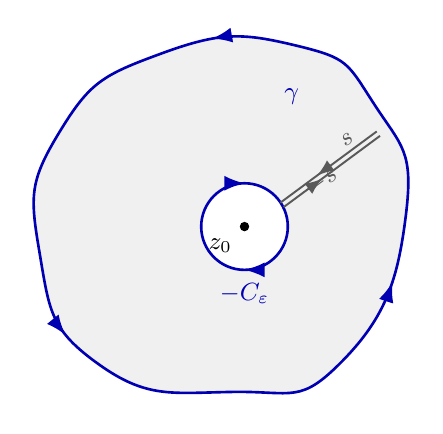
\begin{tikzpicture}[
  >=Latex,
  contour/.style={line width=0.95pt,blue!70!black},
  slit/.style={line width=0.7pt,black!65},
  note/.style={font=\small\sffamily}
]
  \coordinate (Z0) at (0.25,-0.05);

  % Region between the two curves: the integrand is holomorphic here.
  \fill[gray!12,even odd rule]
    plot[smooth cycle,tension=0.9] coordinates {
      (2.30,0.10) (1.90,1.50) (0.90,2.25) (-0.80,2.15) (-2.10,1.15)
      (-2.35,-0.40) (-1.60,-1.80) (0.10,-2.15) (1.50,-1.75) }
    (Z0) circle (0.55);

  % Outer contour gamma, counterclockwise.
  \draw[contour,postaction={decorate},
    decoration={markings,
      mark=at position 0.16 with {\arrow{Latex}},
      mark=at position 0.50 with {\arrow{Latex}},
      mark=at position 0.84 with {\arrow{Latex}}}]
    plot[smooth cycle,tension=0.9] coordinates {
      (2.30,0.10) (1.90,1.50) (0.90,2.25) (-0.80,2.15) (-2.10,1.15)
      (-2.35,-0.40) (-1.60,-1.80) (0.10,-2.15) (1.50,-1.75) };
  \node[note,blue!70!black] at (0.85,1.60) {$\gamma$};

  % Inner circle about z0, traversed clockwise in the combined contour.
  \draw[contour,postaction={decorate},
    decoration={markings,
      mark=at position 0.25 with {\arrow{Latex}},
      mark=at position 0.75 with {\arrow{Latex}}}]
    ($(Z0)+(0.55,0)$) arc[start angle=0,end angle=-180,radius=0.55]
                    arc[start angle=-180,end angle=-360,radius=0.55];
  \node[note,blue!70!black] at ($(Z0)+(0,-0.85)$) {$-C_\varepsilon$};

  % Slit: two antiparallel sides s and -s joining gamma to the circle.
  \coordinate (I) at ($(Z0)+(30:0.55)$);
  \coordinate (O) at (1.95,1.13);
  \draw[slit,postaction={decorate},
    decoration={markings,mark=at position 0.62 with {\arrow{Latex}}}]
    ($(O)+(126.5:0.035)$) -- ($(I)+(126.5:0.035)$);
  \draw[slit,postaction={decorate},
    decoration={markings,mark=at position 0.40 with {\arrow{Latex}}}]
    ($(I)+(306.5:0.035)$) -- ($(O)+(306.5:0.035)$);
  \node[note,black!65,rotate=36.5] at (1.55,1.06) {$s$};
  \node[note,black!65,rotate=36.5] at (1.24,0.52) {$-s$};

  % Evaluation point.
  \fill (Z0) circle (1.7pt) node[note,below left=1pt] {$z_0$};
\end{tikzpicture}
\end{document}
